\section{\textsc{Gurkensalat}}

\subsection*{Zutaten für 2 Portionen:}

\begin{tabular}{p{7.5cm} p{7.5cm}}
	& \\
	\sfrac{1}{2} Gurke & 2EL Olivenöl \\
	1EL Essig & 1TL Zucker \\
	\multicolumn{2}{l}{Salz, Pfeffer, Dill nach Geschmack}
\end{tabular}

\subsection*{Serviervorschlag:}

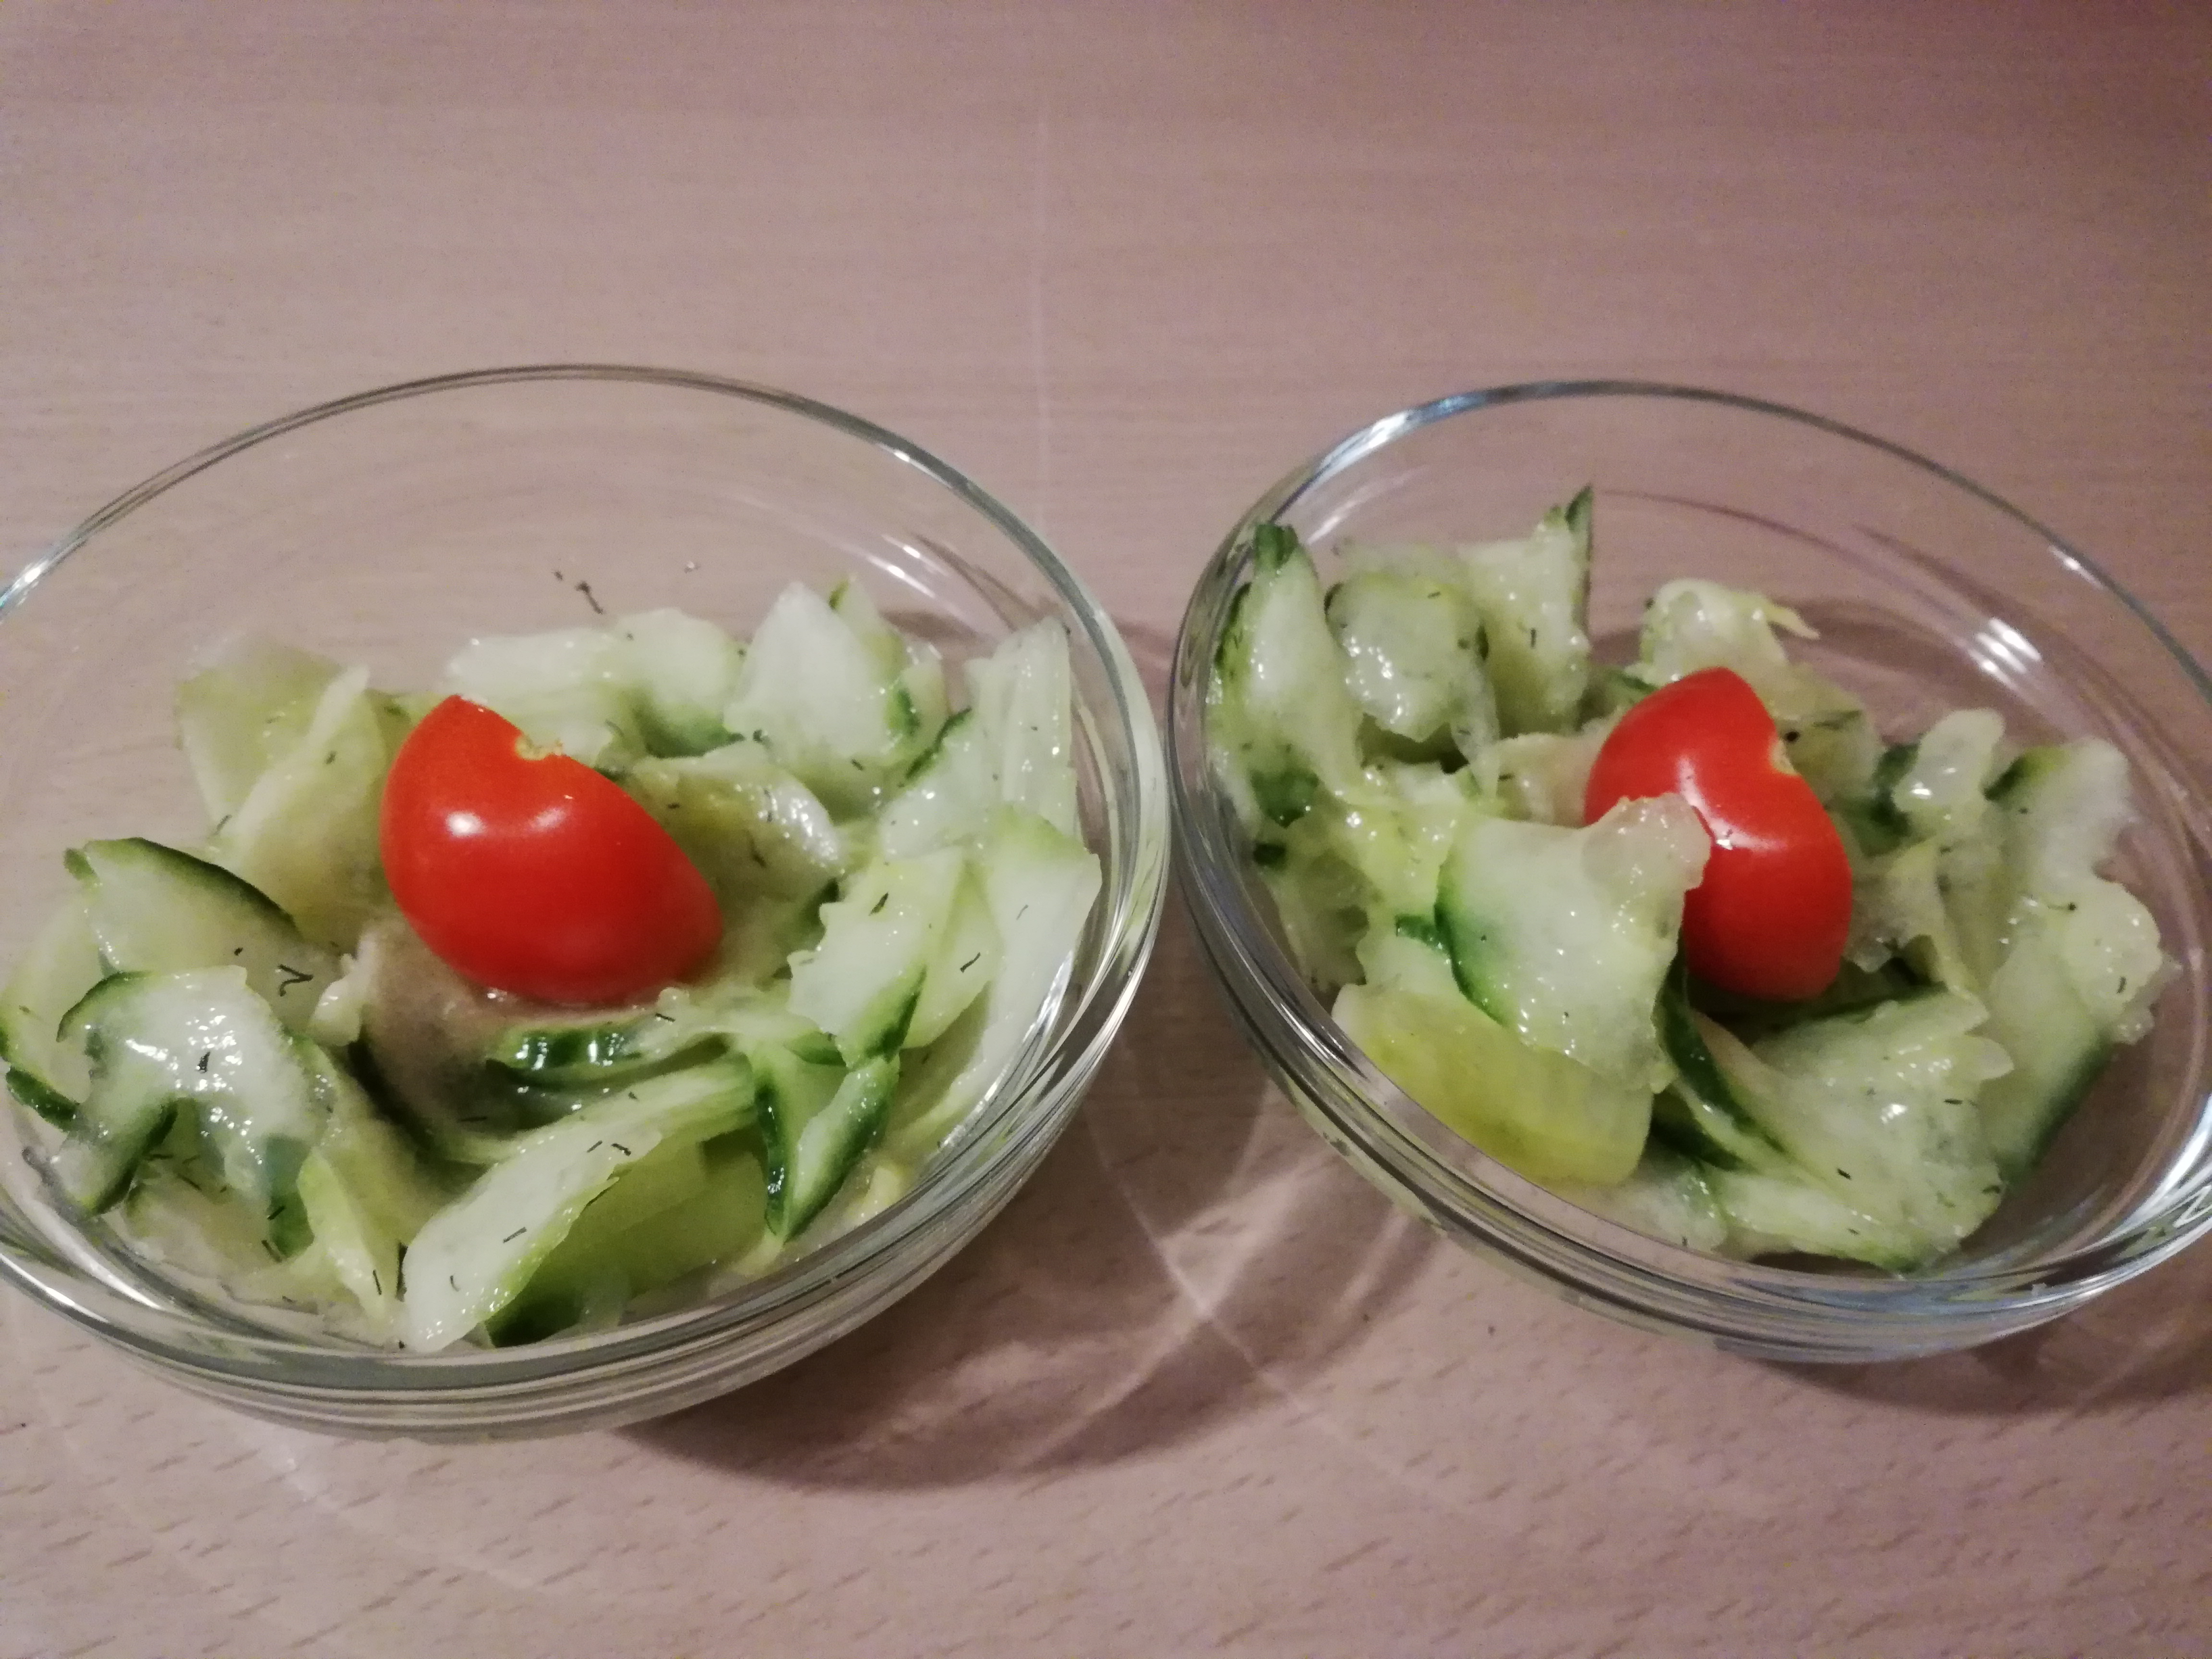
\includegraphics[width=\textwidth]{img/gurkensalat/gurkensalat_fertig.jpg} \cite{gurkensalat}

\subsection*{So geht's:}

\begin{tabular}{p{15cm}}
	\\
	Die Gurke mit einem Sparschäler schälen.\\
	Die geschälte Gurke in feine Streifen schneiden,\\
  oder mit Hilfe einer Küchenreibe in Scheiben reiben.\\
	Die Gewürze und Öle hinzufügen und alles für etwa \sfrac{1}{2}h ziehen lassen.\\
  \textbf{Tipp:} Gurke nur teilweise schälen für farbliche Akzente.
\end{tabular}
